%%%%%%%%%%%%%%%%%%%%%%%%%%%%%%%%%%%%%%%%%
%
% (c) 2022 by Jennifer Laaser
%
% This work is licensed under the Creative Commons Attribution-NonCommercial-ShareAlike 4.0 International License. To view a copy of this license, visit http://creativecommons.org/licenses/by-nc-sa/4.0/ or send a letter to Creative Commons, PO Box 1866, Mountain View, CA 94042, USA.
%
% The current source for these materials is accessible on Github: https://github.com/jlaaser/pogil-polymers
%
%%%%%%%%%%%%%%%%%%%%%%%%%%%%%%%%%%%%%%%%%

\renewcommand{\figpath}{content/polymphys/chain-confs/langevin-chains/figs}
\renewcommand{\labelbase}{langevin-chains}

\begin{activity}[extension]{Elasticity of Real Chains}
\label{\labelbase}

\begin{instructornotes}

	This activity introduces students to the force-extension curves of real chains, as exemplified by the Langevin chain model.
	
	After completing this activity, students will be able to:
			\begin{enumerate}
				\item \dots
			\end{enumerate}
	
			
	\subsection*{Activity summary:}
	\begin{itemize}
		\item \textbf{Activity type:} Learning Cycle
		\item \textbf{Content goals:} See above
		\item \textbf{Process goals:} %https://pogil.org/uploads/attachments/cj54b5yts006cklx4hh758htf-process-skills-official-pogil-list-2015-original.pdf
			\begin{itemize}
				\item Interpreting equations in terms of physical behavior
				\item Reading and interpreting graphs
				\item Oral and written communication of reasoning
			\end{itemize}
		\item \textbf{Duration:} approx. 30 min
		\item \textbf{Instructor preparation required:} 
			\begin{itemize}
				\item None beyond knowledge of relevant content
			\end{itemize}
		\item \textbf{Related textbook chapters:}
			\begin{itemize}
				\item \emph{Polymer Chemistry} (Hiemenz \& Lodge), 2nd ed.: not covered
				\item \emph{Introduction to Polymers} (Young \& Lovell), 3rd ed.: not covered
				\item \emph{Polymer Physics} (Rubinstein \& Colby): Section 2.6.2
			\end{itemize}
	\end{itemize}

\end{instructornotes}

	%\textbf{Focus question:} Put a central question for the students to consider through this exercise here.


\begin{model}[Stretching a Chain to Near its Contour Length]
\label{\labelbase:model:chainstretching}

	An example of a freely-jointed chain with links of length $b$ is shown below:
	
	\vspace{6pt}
	\centerline{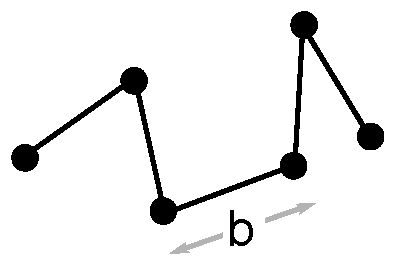
\includegraphics[width=0.3\textwidth]{\figpath/Model1_FJC.pdf}}

\end{model}

%\vspace{0.25in}
\begin{ctqs}

	\question Suppose a freely-jointed chain has exactly 5 links of length $b$.
	
		\begin{enumerate}
			\item Sketch the conformation of this chain in its fully extended state, e.g. when the two ends of the chain are as far away from each other as possible.
			
				\begin{solution}[0.5in]
				\end{solution}
			
			\item How long is the chain in its fully-extended state?
			
				\begin{solution}[0.5in]
				\end{solution}
			
			\item If the links are rigid and cannot stretch, is it physically possible for this chain to have an end-to-end distance longer than the value you calculated in part (b)?  Explain your group's reasoning in 1-2 complete sentences.
			
				\begin{solution}[1.75in]
				\end{solution}
			
		\end{enumerate}
		
	\question More generally, consider a freely-jointed chain with $N$ rigid links of length $b$.
	
		\begin{enumerate}
		
			\item How long would this chain be in its fully-extended state?
			
				\begin{solution}[0.5in]
				\end{solution}
			
			\item If the links are rigid and cannot stretch, is it physically possible for this chain to have an end-to-end distance longer than the value you calculated in part (a)?
			
				\begin{solution}[0.5in]
				\end{solution}
			
			\item Based on your answer to the preceding questions, critique or defend the following statement in 2-3 complete sentences: \label{\labelbase:ctq:probgtNb}
			
				\emph{``The probability of finding a chain with $N$ rigid links of length $b$ at any end-to-end distance greater than $Nb$ must be zero.''}
			
				\begin{solution}[1.5in]
				\end{solution}
			
		\end{enumerate}
	
\end{ctqs}

\begin{infobox}
	In Activity 7.1, we learned that the conformations of freely-jointed chains should follow a Gaussian distribution given by
	\begin{equation*}
		P(N,\vec h_0) = A e^{-\frac{3 h_0^2}{2 N b^2}}
	\end{equation*}
	where $P(N,\vec h_0)$ is the probability of finding a chain with end-to-end vector $\vec h_0$,  $h_0$ is the length of the end-to-end vector (or, distance between the chain ends), and $A$ is a proportionality constant.
	
\end{infobox}

\begin{ctqs}
		
		\question Using this equation, write down expressions for the probability of finding a chain with $N$ links of length $b$ as having each of the following end-to-end distances:
		
			\begin{enumerate}
			
				\item $h_0$ = 0:
			
				\begin{solution}[0.25in]
				\end{solution}
				
				\item $h_0 = \frac{Nb}{2}$:
			
				\begin{solution}[0.25in]
				\end{solution}
				
				\item $h_0 = Nb$:
			
				\begin{solution}[0.25in]
				\end{solution}
				
				\item $h_0 = \frac{3Nb}{2}$:
			
				\begin{solution}[0.25in]
				\end{solution}
				
			\end{enumerate}
			
		\question Are these probabilities consistent with your answer to CTQ \ref{\labelbase:ctq:probgtNb}?  If not, which values disagree?
			
				\begin{solution}[1in]
				\end{solution}

\end{ctqs}

%\begin{model}[The Langevin Chain]
%\label{\labelbase:mdl:langevin}
	
%	As you found in Model \ref{\labelbase:mdl:chainstretching}, the Gaussian distribution only accurately describes the conformations of polymer chains at low extensions (that is, when the end-to-end distance $h_0 << Nb$).
%	
%	It is possible to show that the probability of finding a freely-jointed chain at end-to-end distance $h_0$ is more accurately given by
%	\begin{equation*}
%		P(N,h_0) = A e^{-N\left(\frac{h_0}{Nb}\beta + \ln\frac{\beta}{\sinh\beta}\right)}
%	\end{equation*} 
%	where $\beta = \mathcal{L}^{-1}\left(\frac{h_0}{Nb}\right)$ and $\mathcal{L}^{-1}$ is the so-called ``inverse Langevin function'', which has the following shape:
%	
%	IMAGE
%	
%	The corresponding force-extension relationship is
%	\begin{equation*}
%		f = \frac{kT}{b} \mathcal{L}^{-1}\left(\frac{h}{Nb}\right)
%	\end{equation*}
%\end{model}

\begin{model}
\label{\labelbase:mdl:gaussfd}

	As you learned in Activity 7.2, the force-extension relationship for a Gaussian chain is
	
	\begin{minipage}[c]{0.1\textwidth}
		~
	\end{minipage}
	\begin{minipage}[c]{0.3\textwidth}
	\vspace{0pt}
		\begin{equation*}
			f=\frac{3k_BT}{Nb^2}h
		\end{equation*}
	\end{minipage}
	\begin{minipage}[c]{0.5\textwidth}
	\vspace{0pt}
		\centerline{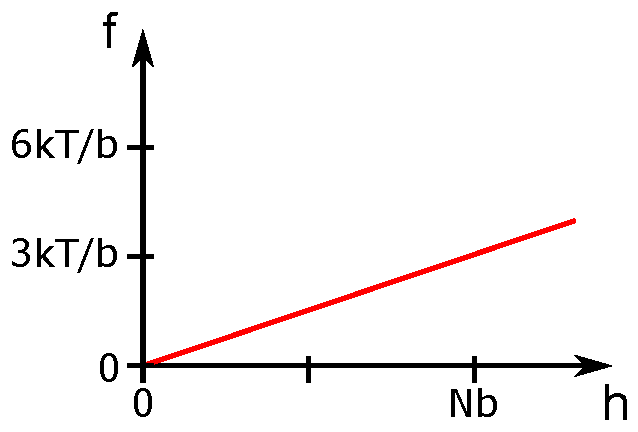
\includegraphics[width=0.8\textwidth]{\figpath/Model2_gaussianFd.pdf}}
	\end{minipage}
	\begin{minipage}[c]{0.1\textwidth}
		~
	\end{minipage}
	
	
\end{model}

\begin{ctqs}
	
	\question If it is \textit{physically impossible} to extend the chain past length $Nb$, what must happen to the force on the chain at this point?
	
		\begin{solution}[1in]
		\end{solution}
	
	\question Sketch the force-distance curve you would expect to measure for a ``real'' chain on the axes below (the Gaussian relationship is shown for reference): \label{\labelbase:ctq:guessrealFd}
		
		\centerline{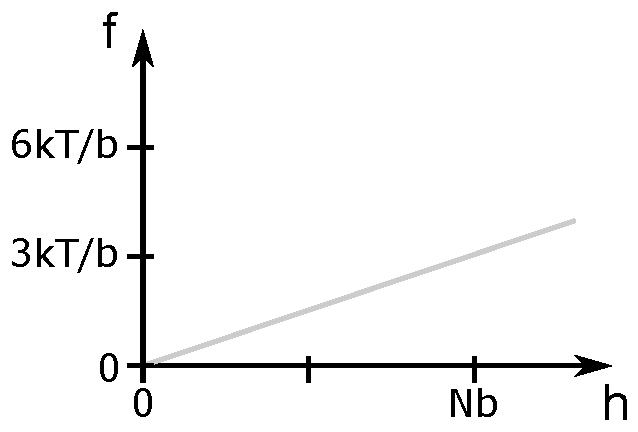
\includegraphics[width=0.45\textwidth]{\figpath/Model2_LangevinFd_blank.pdf}}
	
\end{ctqs}

\begin{infobox}

	It is possible to show %(see Exercise \ref{\labelbase:exc:langevinderivation}) 
	that the force-distance curve for a freely-jointed chain that cannot be extended past its contour length is more accurately given by
	\begin{equation*}
		f = \frac{kT}{b} \mathcal{L}^{-1}\left(\frac{h}{Nb}\right) \label{\labelbase:eqn:Fdlangevin}
	\end{equation*}
	where $\mathcal{L}^{-1}$ is the so-called ``inverse Langevin function''.
	
	The inverse Langevin function has the following shape:
	
	\centerline{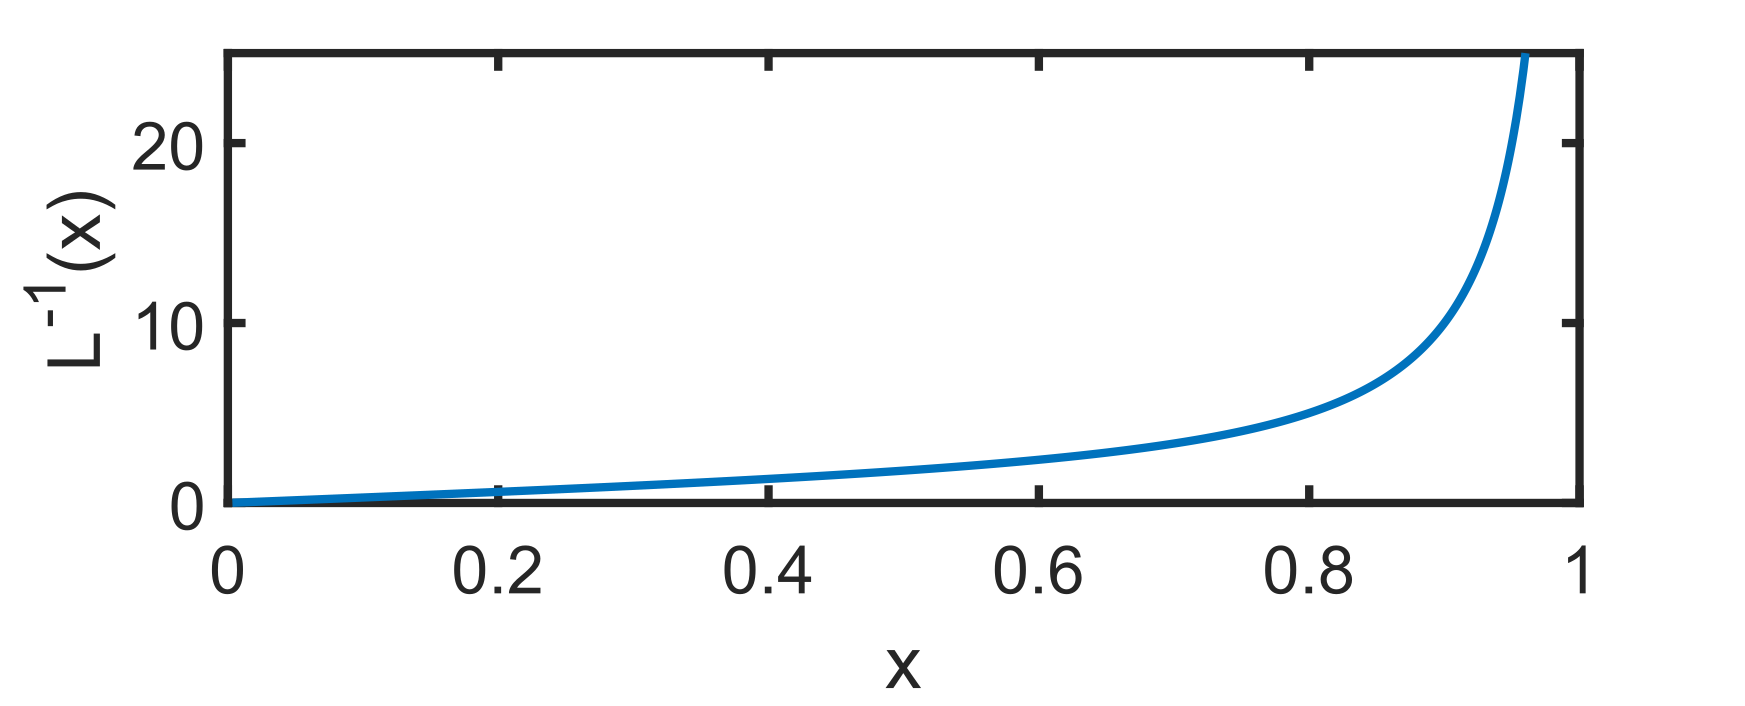
\includegraphics[width=0.5\textwidth]{\figpath/langevin-function.png}}
	
\end{infobox}

\begin{ctqs}
	
	\question Is this functional form consistent with your answer to CTQ \ref{\labelbase:ctq:guessrealFd}?  If not, sketch a more accurate depiction of the force-distance curve for a ``real'' chain on the axes below (the Gaussian force-distance relationship is again shown for reference):
		
		\centerline{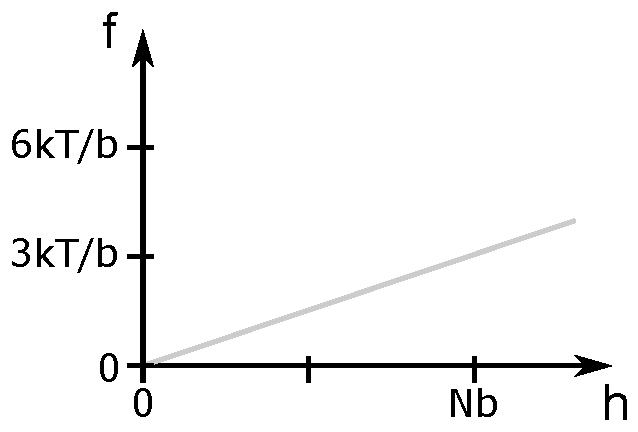
\includegraphics[width=0.45\textwidth]{\figpath/Model2_LangevinFd_blank.pdf}}	
	
	\question The inverse Langevin function can be approximated using a Taylor series expansion as follows:\footnote{see DOI: 10.1007/s00397-014-0802-2}
		\begin{equation*}
			\mathcal{L}^{-1}(x) = 3x + \frac{9}{5}x^3 + \frac{297}{175}x^5 + \dots
		\end{equation*}
		
		\begin{enumerate}
			\item When $x=\frac{h}{Nb}$ is small, why is it reasonable to assume that the $x^3$ and $x^5$ terms make a negligible contribution to the measured force?
			
				\begin{solution}[1in]
				\end{solution}
			
			\item Using $\mathcal{L}^{-1}(x) \approx 3x$, find an expression for the force on a freely-jointed chain with $N$ links of length $b$ in the low extension limit.
			
				\begin{solution}[1.5in]
				\end{solution}
			
		\end{enumerate}
		
	\question Compare your answer to the preceding question to the equation given in Model \ref{\labelbase:mdl:gaussfd}, and use your observations to critique or defend the following statement in 2-3 complete sentences:
	
		\emph{``The Gaussian distribution offers a reasonable description of the conformations and force responses of polymer chains at low extensions, but fails when chains are stretched to extensions approaching their contour lengths.''}
			
				\begin{solution}[2in]
				\end{solution}
	
\end{ctqs}
	

\begin{exercises}

	\exercise Propose a method that you could use to measure the force-distance curve for a single polymer chain.
	
	% something about how this shows up in polymer networks? 
	
%
%\exercise \label{\labelbase:exc:langevinderivation} The force-extension relationship for the Langevin chain given on page \pageref{\labelbase:eqn:Fdlangevin} can be derived as follows:
%
%	\begin{enumerate}
%		\item Find an expression for the potential energy $U(R)$ for a chain extended to 
%	\end{enumerate}
%		
\end{exercises}
	
\end{activity}